\chapter{Affichage et choix des caractères}

	Il faut maintenant réaliser une fonction pour l'affichage et le choix des caractères afin que le joueur puisse saisir une réponse.
    
	Il faut également que cette fonction stocke, de façon pertinente, la réponse du joueur afin qu'une autre fonction puisse en calculer le résultat.
    C'est à dire comparer sa réponse à la solution et dire combien de lettres sont bonnes mais mal positionnées et combien de lettres sont bonnes et bien placées.
	Et qu'entre deux réponses nous ayons la place d'afficher le résultat de la réponse précédente.

\section{Choix de l'algorithme}
	Pour réaliser cette fonction nous avons identifiés plusieurs solution lors de l'étude préalable du programme. 
    Nous avons donc choisi de réaliser une fonction qui enregistrera seulement la réponse actuellement en cours de saisie et qui utilisera la rémanence de l'écran pour conserver les réponses et résultats précédents.
    
    En effet précédemment nous avions remarqué que tant que l'écran n'était pas "nettoyé" l'affichage se conservait dans son état actuel.
    Cette solution simplifiait beaucoup le reste du programme et permettait de limiter les accès mémoire lors de la saisie des réponses et de l'affichage.

\section{Programme}
\underline{Programme utilisé pour tester la fonction de saisie: }
\lstinputlisting{Sources/TestSaisie.ino}

\newpage
\underline{Affichage obtenus lors du test de l'affichage et de la saisie des caractères:}
\begin{figure}[h]
	\centering
   	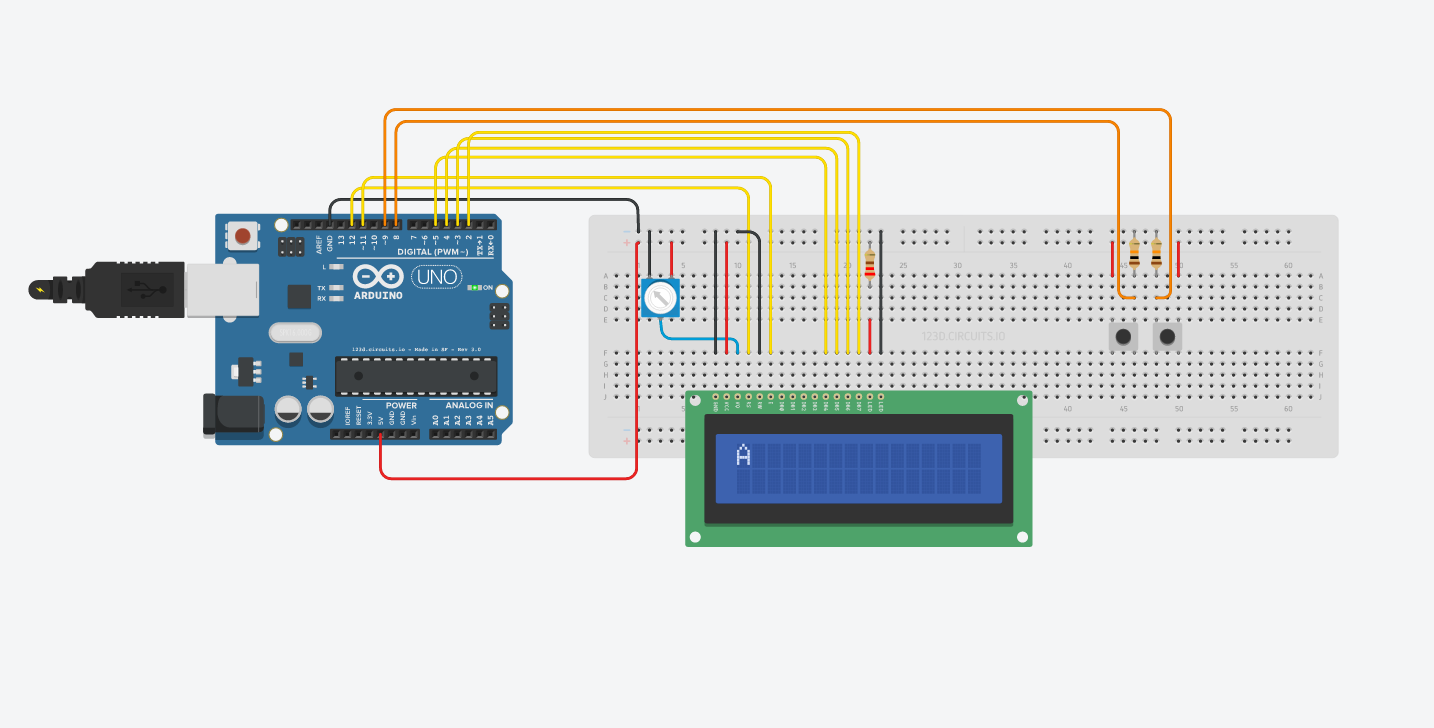
\includegraphics[width=\linewidth]{testSaisie1}
    \caption{Début de la saisie de la 1\iere{} réponse}
    \label{testSaisie1}
\end{figure}

\paragraph{}
Comme nous pouvons le voir sur la figure \ref{testSaisie2} l'affichage est conforme à nos attentes, nous avons bien un espace vide entre deux réponses ainsi qu'un saut a la ligne arrivé au bord de l'écran.
\begin{figure}[h]
	\centering
   	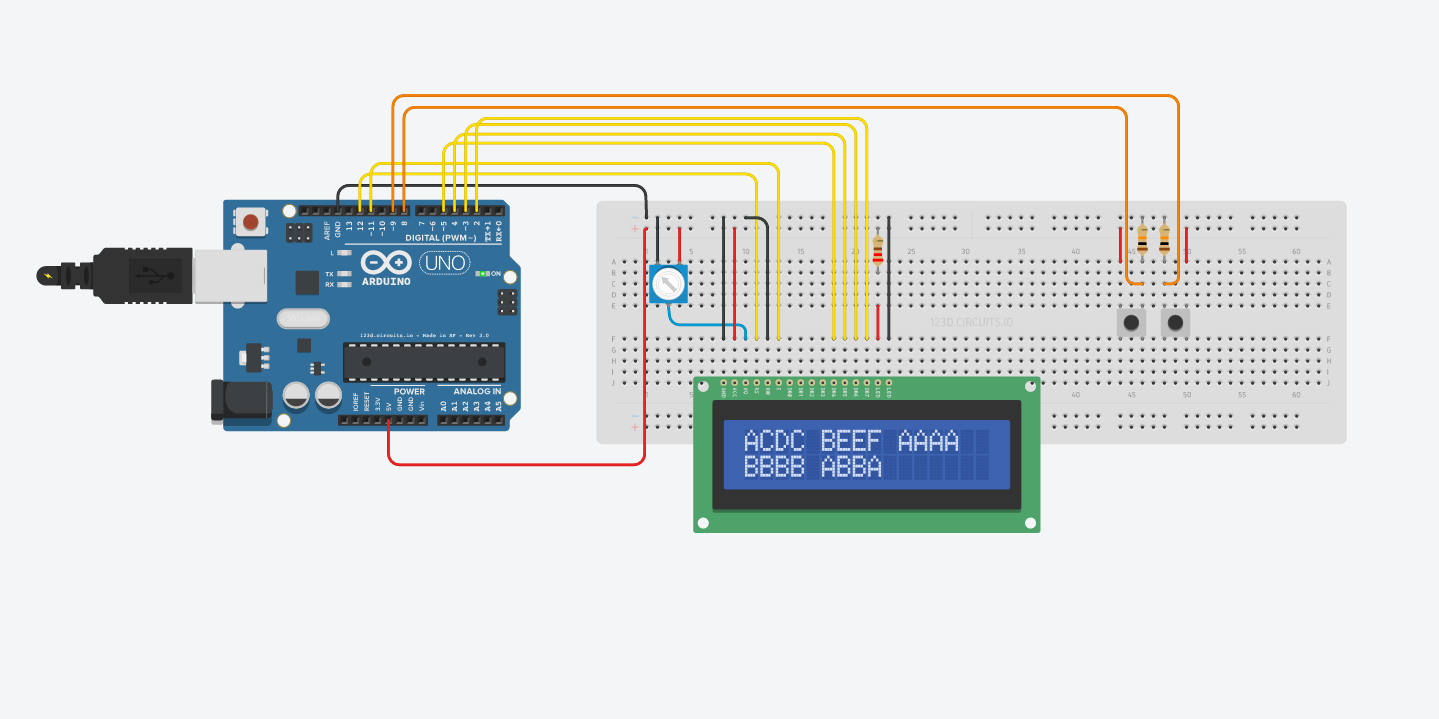
\includegraphics[width=\linewidth]{testSaisie2}
    \caption{Fin de la saisie de la 5\ieme{} réponse}
    \label{testSaisie2}
\end{figure}